% Options for packages loaded elsewhere
\PassOptionsToPackage{unicode}{hyperref}
\PassOptionsToPackage{hyphens}{url}
%
\documentclass[
]{article}
\usepackage{amsmath,amssymb}
\usepackage{iftex}
\ifPDFTeX
  \usepackage[T1]{fontenc}
  \usepackage[utf8]{inputenc}
  \usepackage{textcomp} % provide euro and other symbols
\else % if luatex or xetex
  \usepackage{unicode-math} % this also loads fontspec
  \defaultfontfeatures{Scale=MatchLowercase}
  \defaultfontfeatures[\rmfamily]{Ligatures=TeX,Scale=1}
\fi
\usepackage{lmodern}
\ifPDFTeX\else
  % xetex/luatex font selection
\fi
% Use upquote if available, for straight quotes in verbatim environments
\IfFileExists{upquote.sty}{\usepackage{upquote}}{}
\IfFileExists{microtype.sty}{% use microtype if available
  \usepackage[]{microtype}
  \UseMicrotypeSet[protrusion]{basicmath} % disable protrusion for tt fonts
}{}
\makeatletter
\@ifundefined{KOMAClassName}{% if non-KOMA class
  \IfFileExists{parskip.sty}{%
    \usepackage{parskip}
  }{% else
    \setlength{\parindent}{0pt}
    \setlength{\parskip}{6pt plus 2pt minus 1pt}}
}{% if KOMA class
  \KOMAoptions{parskip=half}}
\makeatother
\usepackage{xcolor}
\usepackage[margin=1in]{geometry}
\usepackage{longtable,booktabs,array}
\usepackage{calc} % for calculating minipage widths
% Correct order of tables after \paragraph or \subparagraph
\usepackage{etoolbox}
\makeatletter
\patchcmd\longtable{\par}{\if@noskipsec\mbox{}\fi\par}{}{}
\makeatother
% Allow footnotes in longtable head/foot
\IfFileExists{footnotehyper.sty}{\usepackage{footnotehyper}}{\usepackage{footnote}}
\makesavenoteenv{longtable}
\usepackage{graphicx}
\makeatletter
\newsavebox\pandoc@box
\newcommand*\pandocbounded[1]{% scales image to fit in text height/width
  \sbox\pandoc@box{#1}%
  \Gscale@div\@tempa{\textheight}{\dimexpr\ht\pandoc@box+\dp\pandoc@box\relax}%
  \Gscale@div\@tempb{\linewidth}{\wd\pandoc@box}%
  \ifdim\@tempb\p@<\@tempa\p@\let\@tempa\@tempb\fi% select the smaller of both
  \ifdim\@tempa\p@<\p@\scalebox{\@tempa}{\usebox\pandoc@box}%
  \else\usebox{\pandoc@box}%
  \fi%
}
% Set default figure placement to htbp
\def\fps@figure{htbp}
\makeatother
\setlength{\emergencystretch}{3em} % prevent overfull lines
\providecommand{\tightlist}{%
  \setlength{\itemsep}{0pt}\setlength{\parskip}{0pt}}
\setcounter{secnumdepth}{-\maxdimen} % remove section numbering
% definitions for citeproc citations
\NewDocumentCommand\citeproctext{}{}
\NewDocumentCommand\citeproc{mm}{%
  \begingroup\def\citeproctext{#2}\cite{#1}\endgroup}
\makeatletter
 % allow citations to break across lines
 \let\@cite@ofmt\@firstofone
 % avoid brackets around text for \cite:
 \def\@biblabel#1{}
 \def\@cite#1#2{{#1\if@tempswa , #2\fi}}
\makeatother
\newlength{\cslhangindent}
\setlength{\cslhangindent}{1.5em}
\newlength{\csllabelwidth}
\setlength{\csllabelwidth}{3em}
\newenvironment{CSLReferences}[2] % #1 hanging-indent, #2 entry-spacing
 {\begin{list}{}{%
  \setlength{\itemindent}{0pt}
  \setlength{\leftmargin}{0pt}
  \setlength{\parsep}{0pt}
  % turn on hanging indent if param 1 is 1
  \ifodd #1
   \setlength{\leftmargin}{\cslhangindent}
   \setlength{\itemindent}{-1\cslhangindent}
  \fi
  % set entry spacing
  \setlength{\itemsep}{#2\baselineskip}}}
 {\end{list}}
\usepackage{calc}
\newcommand{\CSLBlock}[1]{\hfill\break\parbox[t]{\linewidth}{\strut\ignorespaces#1\strut}}
\newcommand{\CSLLeftMargin}[1]{\parbox[t]{\csllabelwidth}{\strut#1\strut}}
\newcommand{\CSLRightInline}[1]{\parbox[t]{\linewidth - \csllabelwidth}{\strut#1\strut}}
\newcommand{\CSLIndent}[1]{\hspace{\cslhangindent}#1}
\usepackage{booktabs}
\usepackage{longtable}
\usepackage{array}
\usepackage{multirow}
\usepackage{wrapfig}
\usepackage{float}
\usepackage{colortbl}
\usepackage{pdflscape}
\usepackage{tabu}
\usepackage{threeparttable}
\usepackage{threeparttablex}
\usepackage[normalem]{ulem}
\usepackage{makecell}
\usepackage{xcolor}
\usepackage{bookmark}
\IfFileExists{xurl.sty}{\usepackage{xurl}}{} % add URL line breaks if available
\urlstyle{same}
\hypersetup{
  pdftitle={Appendix 1: Description of data},
  hidelinks,
  pdfcreator={LaTeX via pandoc}}

\title{Appendix 1: Description of data}
\author{}
\date{\vspace{-2.5em}}

\begin{document}
\maketitle

\section{Appendix 1}\label{appendix-1}

The integrated population model provides a framework for synthesizing
multiple demographic datasets to mutually inform shared parameters. In
Appendix 1.1, we further describe the multi-year Drayton Harbor time
series data (D1). In Appendix 1.2, we describe additional information
about the size-at-age data (D2), and in Appendix 1.3, we further
describe the mark-recapture data (D3).

\subsection{Appendix 1.1}\label{appendix-1.1}

The multi-year time series data (D1) was collected in Drayton Harbor, an
enclosed bay in the Salish Sea in Washington State, USA.

\textbf{Figure A1.1:} Bathymetric map of Drayton Harbor. Colors indicate
depth and black line indicates coast line.

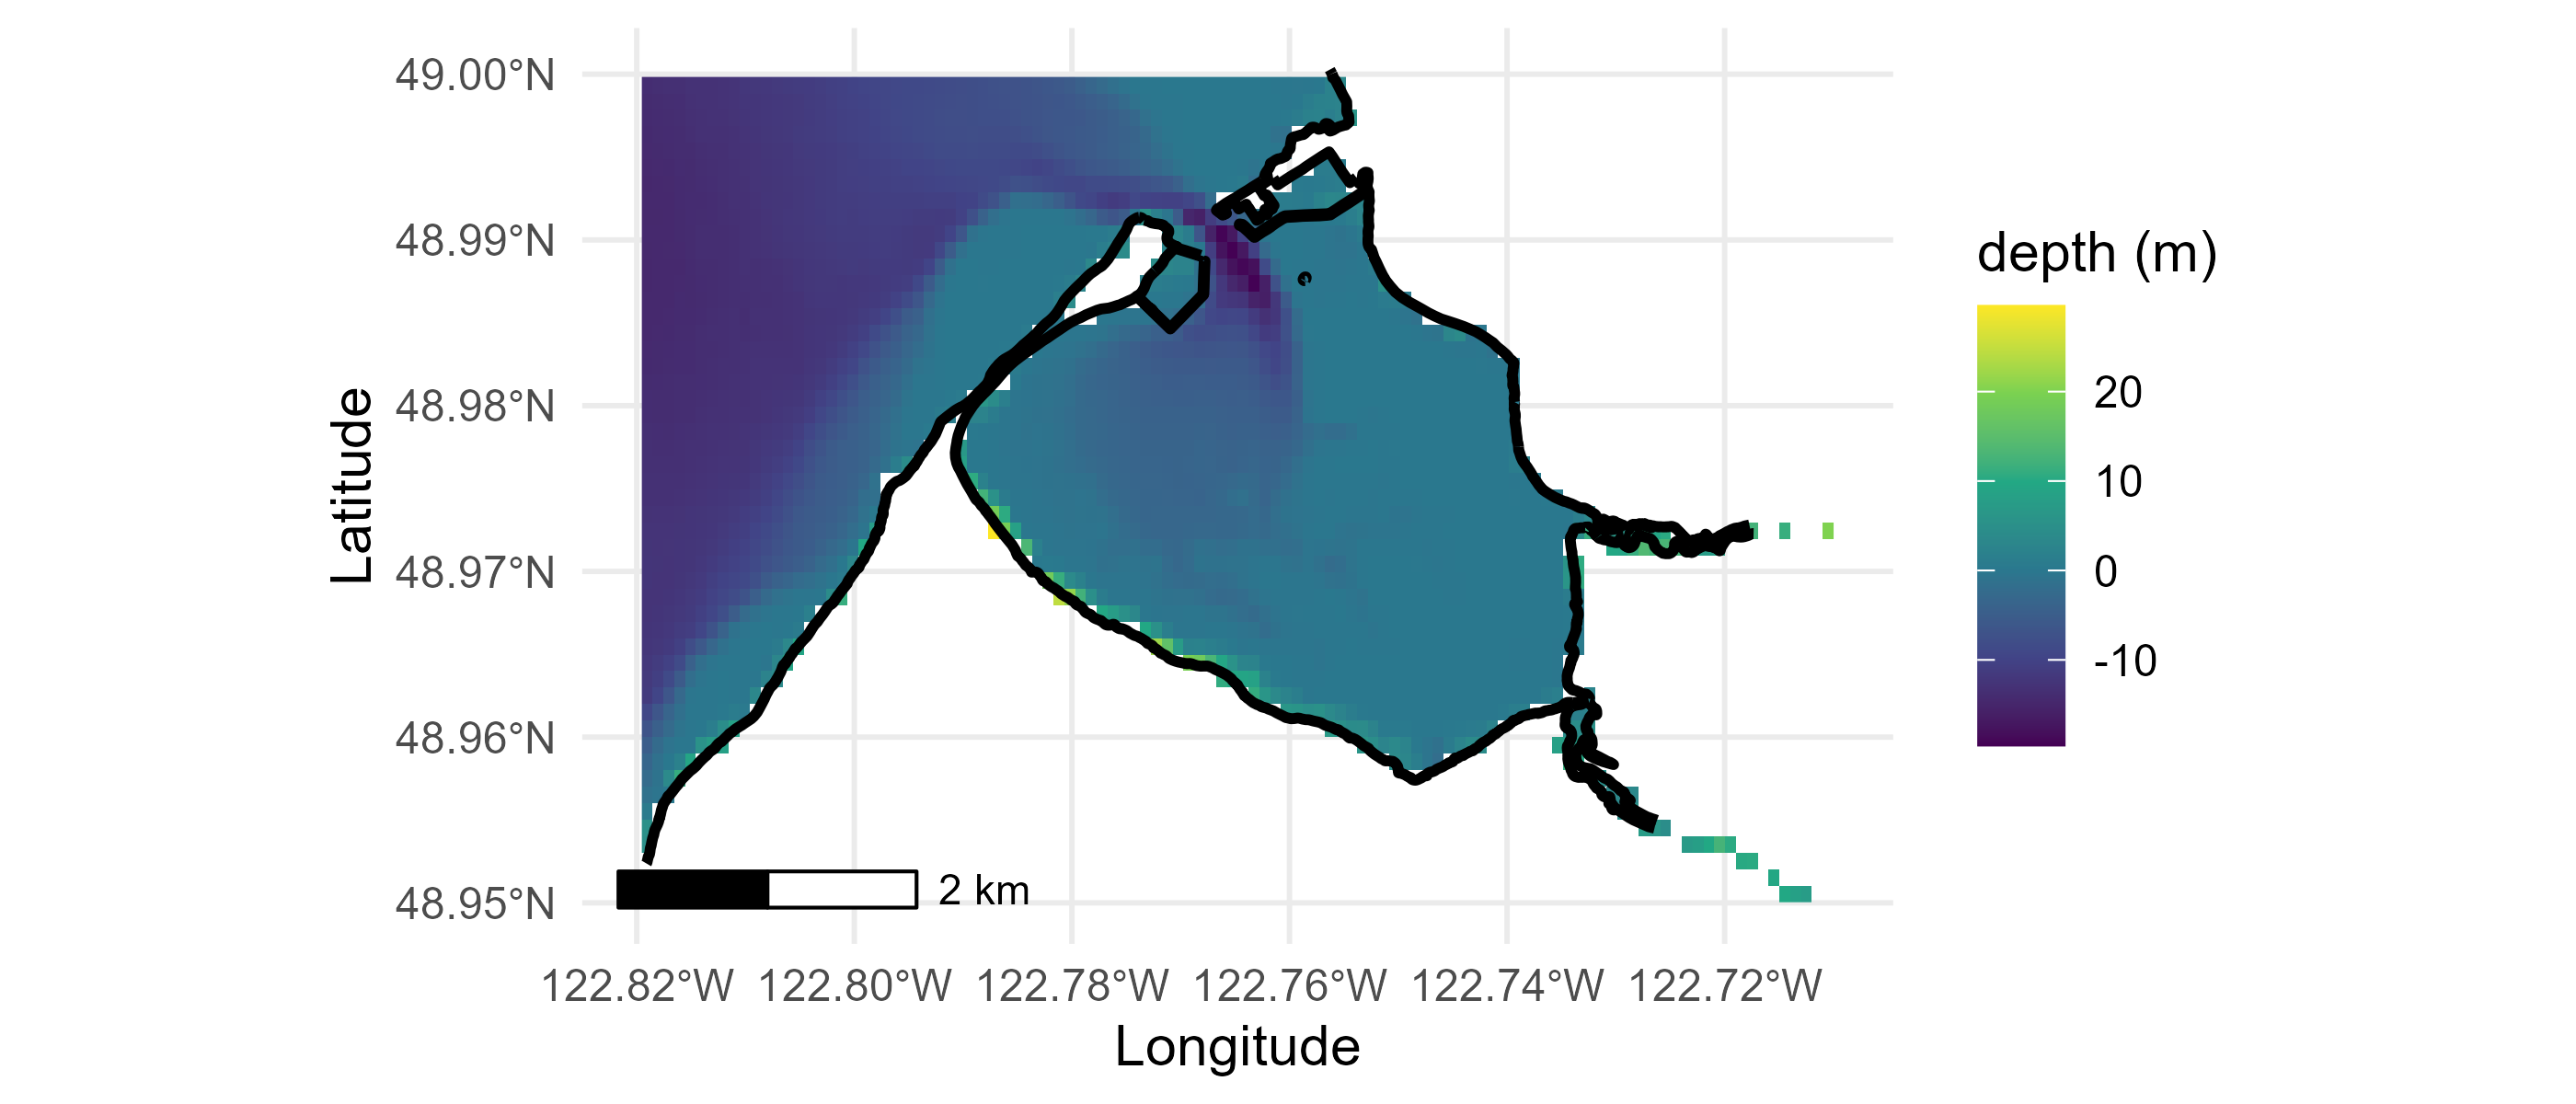
\includegraphics[width=38.89in]{../figures/supplemental_map}

At Drayton Harbor, traps were baited and left to ``soak'' in intertidal
and subtidal habitat for 24-48 hours. Trapped areas within Drayton
Harbor include a large tideflat and the mouth of three creeks that feed
into the bay (named ``North'', ``Dakota Creek'', ``California Creek'',
and ``Noname Creek''). After the ``soak'' time, traps were retrieved,
and green crabs were counted and removed from the system. The carapace
widths (CW) of green crabs were measured with vernier calipers between
the tips of their fifth anterio-lateral spines to the nearest lowest mm.
Multiple trap types (Fukui, Minnow, and Shrimp) with different
size-selective removal rates were used. These traps have different mesh
sizes and entrance openings: Fukui traps have 12 mm mesh with
approximately 20 cm entrance openings; Gee-brand minnow traps have 6 mm
mesh with approximately 5 cm entrances; Promar-brand 4-way Shrimp traps
have 12.7 mm or 25.4 mm mesh size and approximately 10 cm entrance
opening.

Data collected in Drayton Harbor data were subset to only include
recruits (age \textless{} 1) that appear in a single cohort in the fall
of each year (Figure 1B). This subset only removed three recruit
individuals in 2022 from the dataset that were from an off-cycle
recruitment cohort.

Below we describe the total removal effort and catch of European green
crab (EGC, \emph{C. maenas}) in Drayton Harbor (D1). While the removal
count data is collected at many time points throughout the trapping
season (April - October), we discretize the time intervals into biweekly
periods in the model.

\newpage

\textbf{Table A1.1:} Number of crabs caught and total removal effort
(number of traps) during each biweek and year. Julian day signifies the
first Julian day of the discretized biweek period. F, M, and S
correspond to Fukui, Minnow, and Shrimp traps, respectively.

\begin{longtable}[]{@{}
  >{\raggedleft\arraybackslash}p{(\linewidth - 14\tabcolsep) * \real{0.1392}}
  >{\raggedright\arraybackslash}p{(\linewidth - 14\tabcolsep) * \real{0.0633}}
  >{\raggedright\arraybackslash}p{(\linewidth - 14\tabcolsep) * \real{0.1266}}
  >{\raggedright\arraybackslash}p{(\linewidth - 14\tabcolsep) * \real{0.1392}}
  >{\raggedright\arraybackslash}p{(\linewidth - 14\tabcolsep) * \real{0.1266}}
  >{\raggedright\arraybackslash}p{(\linewidth - 14\tabcolsep) * \real{0.1392}}
  >{\raggedright\arraybackslash}p{(\linewidth - 14\tabcolsep) * \real{0.1266}}
  >{\raggedright\arraybackslash}p{(\linewidth - 14\tabcolsep) * \real{0.1392}}@{}}
\toprule\noalign{}
\begin{minipage}[b]{\linewidth}\raggedleft
Julian day
\end{minipage} & \begin{minipage}[b]{\linewidth}\raggedright
year
\end{minipage} & \begin{minipage}[b]{\linewidth}\raggedright
F (catch)
\end{minipage} & \begin{minipage}[b]{\linewidth}\raggedright
F (effort)
\end{minipage} & \begin{minipage}[b]{\linewidth}\raggedright
M (catch)
\end{minipage} & \begin{minipage}[b]{\linewidth}\raggedright
M (effort)
\end{minipage} & \begin{minipage}[b]{\linewidth}\raggedright
S (catch)
\end{minipage} & \begin{minipage}[b]{\linewidth}\raggedright
S (effort)
\end{minipage} \\
\midrule\noalign{}
\endhead
\bottomrule\noalign{}
\endlastfoot
137 & 2020 & 12 & 48 & 22 & 43 & 0 & 0 \\
152 & 2020 & 16 & 67 & 10 & 62 & 0 & 0 \\
167 & 2020 & 8 & 62 & 5 & 57 & 0 & 0 \\
182 & 2020 & 4 & 100 & 0 & 96 & 0 & 0 \\
198 & 2020 & 1 & 64 & 0 & 44 & 0 & 0 \\
213 & 2020 & 12 & 61 & 0 & 60 & 0 & 0 \\
229 & 2020 & 7 & 82 & 0 & 71 & 0 & 0 \\
244 & 2020 & 8 & 97 & 4 & 87 & 0 & 0 \\
259 & 2020 & 4 & 15 & 0 & 10 & 0 & 0 \\
259 & 2020 & 15 & 57 & 23 & 52 & 0 & 0 \\
91 & 2021 & 1 & 180 & 4 & 180 & 0 & 0 \\
106 & 2021 & 7 & 168 & 1 & 168 & 0 & 0 \\
121 & 2021 & 8 & 130 & 2 & 130 & 0 & 0 \\
137 & 2021 & 9 & 207 & 2 & 205 & 0 & 0 \\
152 & 2021 & 4 & 180 & 0 & 180 & 0 & 0 \\
167 & 2021 & 6 & 198 & 0 & 198 & 0 & 0 \\
182 & 2021 & 2 & 120 & 0 & 120 & 0 & 0 \\
198 & 2021 & 0 & 123 & 0 & 123 & 0 & 0 \\
213 & 2021 & 18 & 200 & 0 & 203 & 0 & 0 \\
229 & 2021 & 1 & 251 & 1 & 251 & 12 & 27 \\
244 & 2021 & 8 & 296 & 3 & 297 & 27 & 39 \\
259 & 2021 & 0 & 0 & 0 & 60 & 23 & 24 \\
106 & 2022 & 0 & 135 & 0 & 135 & 3 & 12 \\
121 & 2022 & 2 & 195 & 0 & 195 & 13 & 17 \\
137 & 2022 & 0 & 90 & 0 & 90 & 4 & 12 \\
152 & 2022 & 0 & 127 & 1 & 125 & 4 & 16 \\
167 & 2022 & 2 & 120 & 0 & 120 & 22 & 27 \\
182 & 2022 & 0 & 0 & 0 & 0 & 4 & 6 \\
198 & 2022 & 0 & 62 & 1 & 62 & 15 & 23 \\
213 & 2022 & 0 & 207 & 0 & 207 & 20 & 71 \\
229 & 2022 & 0 & 30 & 0 & 30 & 6 & 50 \\
244 & 2022 & 0 & 0 & 0 & 0 & 5 & 26 \\
259 & 2022 & 0 & 0 & 2 & 26 & 23 & 25 \\
259 & 2022 & 7 & 27 & 29 & 118 & 37 & 50 \\
290 & 2022 & 0 & 0 & 0 & 0 & 6 & 12 \\
305 & 2022 & 8 & 30 & 16 & 30 & 16 & 10 \\
106 & 2023 & 0 & 120 & 2 & 120 & 3 & 20 \\
121 & 2023 & 2 & 163 & 1 & 163 & 20 & 31 \\
137 & 2023 & 2 & 95 & 2 & 95 & 23 & 34 \\
152 & 2023 & 0 & 0 & 0 & 0 & 12 & 26 \\
167 & 2023 & 5 & 60 & 2 & 60 & 8 & 28 \\
182 & 2023 & 0 & 80 & 2 & 80 & 18 & 14 \\
198 & 2023 & 0 & 60 & 0 & 60 & 2 & 26 \\
213 & 2023 & 0 & 43 & 2 & 45 & 2 & 22 \\
229 & 2023 & 0 & 72 & 0 & 149 & 6 & 31 \\
244 & 2023 & 0 & 15 & 0 & 45 & 0 & 18 \\
259 & 2023 & 0 & 30 & 1 & 105 & 10 & 30 \\
259 & 2023 & 0 & 0 & 0 & 0 & 0 & 6 \\
290 & 2023 & 1 & 45 & 1 & 90 & 14 & 112 \\
\end{longtable}

\newpage

\subsection{Appendix 1.2}\label{appendix-1.2}

Size-at-age data (D2) were collected from crab removal observations
associated with range expansions in northeastern Pacific estuaries
documented by Yamada et al.~2021. Since the colonizing cohorts of crabs
following expansion events were relatively easy to identify as they age
over time, Yamada et al.~2021 assigned a year class to captured crabs
based on the location of collection, assumed expansion event, date of
capture, carapace width, sex, and molt conditions (Yamada et al. 2021).

For example, El Niño events, with their characteristic warm water
temperatures and enhanced northward transport by the Davidson Current,
are especially favorable to the survival and transport of larvae
hundreds of kilometers from source populations. The 1997 to 1998 El Niño
resulted in the colonization of embayments in Oregon, coastal
Washington, and on the west coast of Vancouver Island from California,
and the El Niño of 2015 to 2016 and the Pacific Warm Blob were linked to
range expansion into the Salish Sea. More local range expansions in
other areas also occurred during non-El Niño years.

Yamada et al.~2021 report an estimated year class for captured crabs,
which corresponds to the first year of growth after settlement from its
planktonic larval stage. We use this estimated year class and the
reported crab capture date from this dataset to estimate the age of
captured individuals. We assume planktonic settlement in March. For
example, for a crab captured in September 2000 with estimated year class
of 1998 would be assigned an age of 2.5.

\textbf{Table A1.2:} Number of size-at-age records during each year and
waterbody in the northeastern Pacific.

\begin{longtable}[]{@{}rlr@{}}
\toprule\noalign{}
Year & Waterbody & n \\
\midrule\noalign{}
\endhead
\bottomrule\noalign{}
\endlastfoot
1995 & Humboldt Bay & 2 \\
1997 & Coos Bay & 2 \\
1998 & Yaquina Bay & 1 \\
1999 & Barkley Sound & 2 \\
1999 & Price Bay & 1 \\
2000 & Clayoquot Sound & 1 \\
2000 & Nootka Sound & 1 \\
2001 & Little Espinosa Inlet & 3 \\
2007 & Klaskino Inlet & 1 \\
2011 & Gale Passage & 2 \\
2015 & Kildidt Inlet & 2 \\
2016 & Higgins Passage & 1 \\
2016 & Westcott Bay & 1 \\
2017 & Becher Bay & 3 \\
2017 & Padilla Bay & 1 \\
2017 & Whidbey Island & 2 \\
2018 & Port Townshend Bay & 1 \\
2018 & Scow Bay & 1 \\
2018 & Westcott Bay & 2 \\
2018 & Whidbey Island & 1 \\
2018 & Witty's Lagoon & 1 \\
2019 & Bellingham & 3 \\
2019 & Boundary Bay & 3 \\
2019 & Chuckanut Bay & 1 \\
2019 & Esquimalt Lagoon & 2 \\
2019 & Lummi Bay & 2 \\
2019 & Salt Spring Island & 4 \\
2019 & Samish Bay & 1 \\
2019 & Sequim Bay & 3 \\
2019 & Westcott Bay & 1 \\
2019 & Witty's Lagoon & 2 \\
2020 & Chuckanut Bay & 1 \\
2020 & Daajing Giids & 1 \\
\end{longtable}

\subsubsection{Appendix 1.3}\label{appendix-1.3}

The mark-recapture data (D3) were collected as part of a mark-recapture
experiment in July through November 2024 at Roche Cove on Vancouver
Island in British Columbia, Canada.

Green crab were trapped using baited Fukui traps, with trap lines
consisting of six traps placed 10 meters apart. Lines were set
approximately 10 m apart and set both parallel and perpendicular to the
shore line to create an equal grid across the site, and traps ``soaked''
for about 24 hours before being checked. Captured crabs were measured,
sexed, and color and health determined before marking. All crab were
tagged using small sequentially numbered disk tags, with the edges
trimmed down to size, glued to the hind end of the carapace using Crazy
Glue, with accelerant sprayed lightly on to set. Crab were held in
submerged sealed Fukui traps for 24-48 hours and, prior to release, the
tags were individually checked for retention. Crab were evenly dispersed
throughout the trapping location to ensure equal re-distribution across
the site.

The experiment took place over four time periods, \(t \in \{0 ... 3\}\).
Marking events took place at \(t \in \{0 ... 2\}\), where crabs were
marked and released back into the environment. Recapture events took
place at \(t \in \{1 ... 3\}\), and recaptured crabs at
\(t \in \{1,  2\}\) were released back into the environment (Figure
A1.2).

\textbf{Figure A1.2:} Conceptual diagram of mark-recapture schema. The
number of crabs marked at time \(t\) of size \(x\) is
\(m^{\text{mc}}_t(x)\), the number of crabs recaptured at time \(t\) of
size \(x\) is \(r^{\text{mc}}_t(x)\), and the total number of crabs
marked at time \(t\) of size \(x\) is \(N^{\text{mc}}_t(x)\).

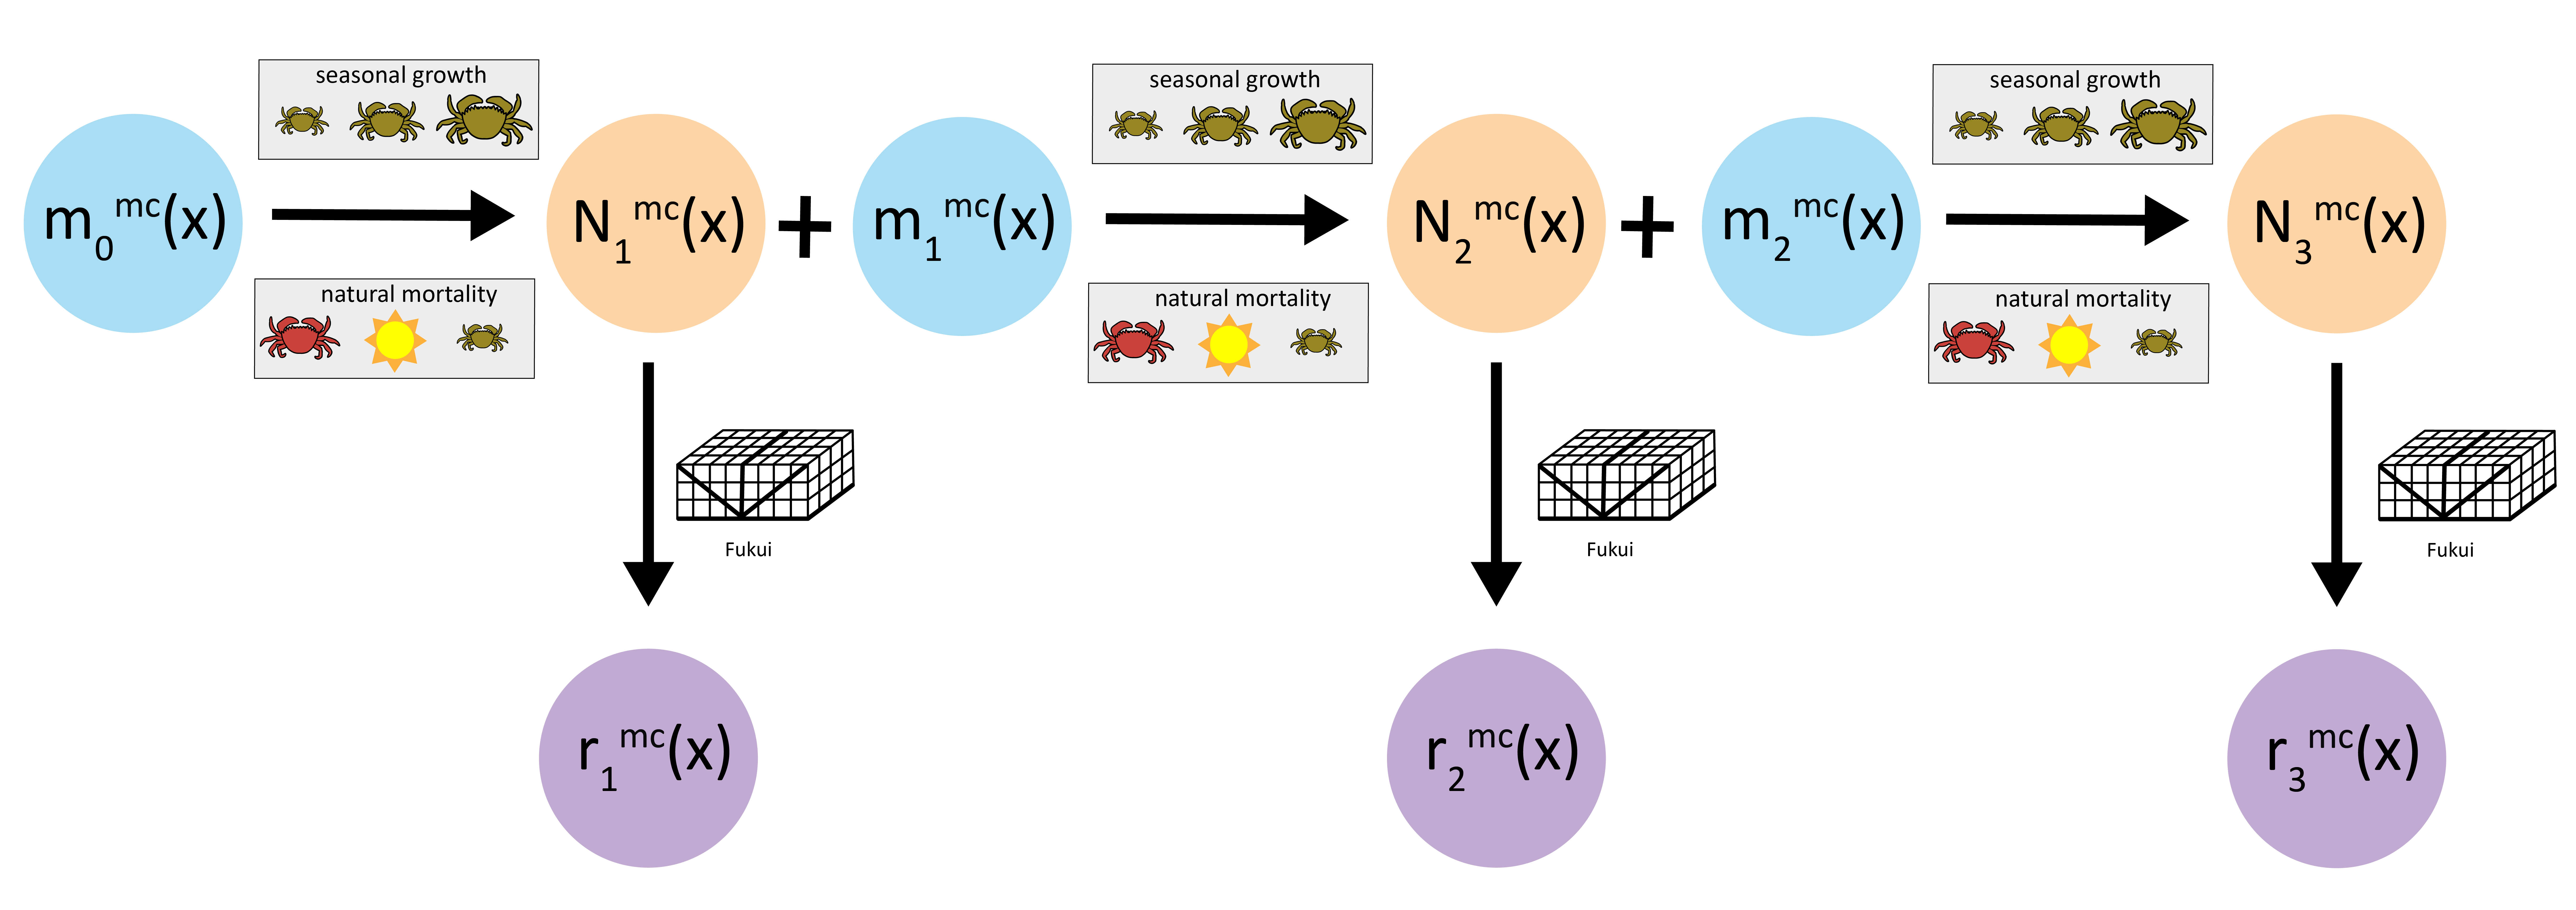
\includegraphics[width=136.25in]{../figures/appendix_mark_recapture_conceptual-01}

Across the four time periods, 234 total traps were set, 1676 crabs were
marked, and 88 crabs were recaptured (Table A1.3).

\textbf{Table A1.3:} Total number of Fukui traps set, crabs marked
(across all sizes), and crabs recaptured (across all sizes) for each of
the four mark-recapture time periods.

\begin{longtable}[]{@{}rrrrr@{}}
\toprule\noalign{}
t & Julian day & Total traps set & Total marked & Total recaptured \\
\midrule\noalign{}
\endhead
\bottomrule\noalign{}
\endlastfoot
0 & 197 & 36 & 590 & NA \\
1 & 213 & 54 & 558 & 23 \\
2 & 244 & 54 & 528 & 37 \\
3 & 305 & 90 & NA & 28 \\
\end{longtable}

\section*{References}\label{references}
\addcontentsline{toc}{section}{References}

\phantomsection\label{refs}
\begin{CSLReferences}{1}{0}
\bibitem[\citeproctext]{ref-yamada2021ocean}
Yamada, Sylvia Behrens, Graham E Gillespie, Richard E Thomson, and Tammy
C Norgard. 2021. {``Ocean Indicators Predict Range Expansion of an
Introduced Species: Invasion History of the European Green Crab Carcinus
Maenas on the North American Pacific Coast.''} \emph{Journal of
Shellfish Research} 40 (2): 399--413.

\end{CSLReferences}

\end{document}
